\documentclass[11pt,letterpaper]{article}

\usepackage{graphicx}
\usepackage[margin=1in]{geometry}
\usepackage{amsmath}
\usepackage[T1]{fontenc}
\usepackage[utf8]{inputenc}
\usepackage{authblk}
\usepackage{fancyhdr}
\usepackage{lastpage}
\usepackage[parfill]{parskip}
\usepackage{subcaption}

\pagestyle{fancyplain}

% Headers
\lhead{}
\chead{}
\rhead{}

% Footers
\lfoot{}
\cfoot{}
\rfoot{\footnotesize Page \thepage\ of \pageref{LastPage}}

\renewcommand{\headrulewidth}{0.0pt} % No header rule
\renewcommand{\footrulewidth}{0.4pt} % Thin footer rule

\title{Consistency Simulations: Raft vs. Eventual (High Conflict)}
\date{August 26, 2016}
\author[ ]{Benjamin Bengfort}
\author[ ]{Pete Keleher}
\affil[ ]{Department of Computer Science}
\affil[ ]{University of Maryland}
\affil[ ]{\textit{\{bengfort,keleher\}@cs.umd.edu}}

\begin{document}

\maketitle

These results present the Eventual vs. Raft homogenous systems with increasing number of nodes in a higher conflict environment than the August 25, 2016 version of the results. The $P_{conflict}$ has been increased from 0.5 to 0.8 and the number of objects reduced from 30 to 10, which has caused a shift in the average number of accesses per object (per device) to increase from 80 to 240. These and other simulation settings are specified in Table \ref{table:settings}. The point of increasing conflict was to more fully explore the relationship of Raft and Eventual to \textit{forked writes} (Figure \ref{fig:forked_writes}) and \textit{stale reads} (Figure \ref{fig:stale_reads}) as the number of nodes increases.

The percent of reads that are stale are roughly equivalent in both Raft and Eventual as shown in Figure \ref{fig:stale_reads}, though eventual starts to do slightly worse than Raft the more nodes are added. Because of bilateral anti-entropy sessions, full convergence time is approximately $t_{visibility} \approx \frac{T}{4} \log_3N$ where $N$ is the number of nodes and $T$ is the tick parameter. For Raft, convergence time is the heartbeat interval, $t_{visibility} \approx \frac{T}{2}$ when all writes are broadcasted to the entire system (these numbers are approximated due to random selection, variable latency, and remote vs local write latency) these approximations are shown next to the real measurements in Figure \ref{fig:visibility_latency}. If we assume that convergence is the primary factor in reducing stale reads, then Raft should do a lot better \textit{after 9 nodes}, however given that after 25 nodes almost all reads are stale and that less than 10\% of writes become fully visible, I would say that stale reads are dependent on the average latency to the maximum visibility of a write. Note that the average visibility for a write is given in Figure \ref{fig:mean_visibility} and the mean latency for the maximal replication of a write is given in Figure \ref{fig:partial_visibility_latency}. This graph shows that the maximal convergence latency for eventual is no worse than twice that of Raft, and might be an explanation for why Eventual only has marginally more stale reads.

The percent of writes that are forks is much higher in Raft than eventual as shown in Figure \ref{fig:forked_writes}. This is because Raft does not allow forks, so any conflict that occurs within a heartbeat interval will be a fork, only one single writer (the first received by the leader in a remote write or the leader itself) will not fork, all other writes to that object in the heartbeat interval will be a fork. On the other hand, while a single fork can occur in Eventual, branches can be extended from that fork without conflict. Since the convergence delay is longer, there is less opportunity to fork and more opportunity to branch. \textbf{Note:} Pete has suggested a metric of \textit{stale writes} to explore this issue more.

\begin{figure}[!h]
    \centering
        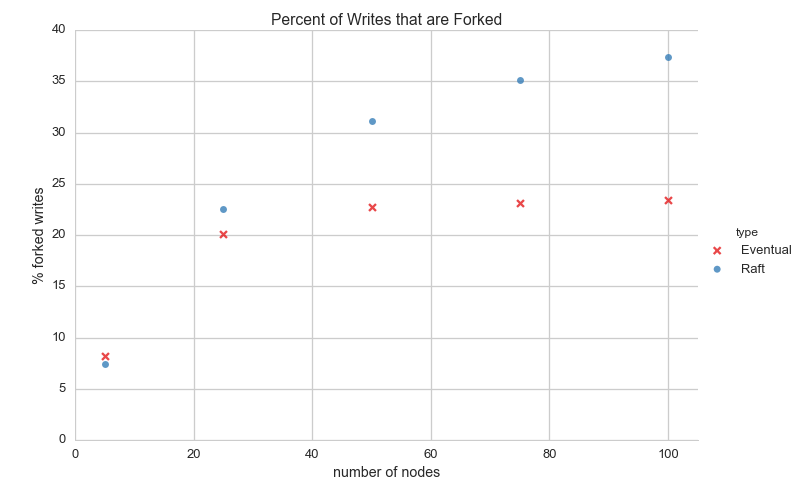
\includegraphics[width=\textwidth]{hcfigures/forked_writes.png}
        \caption{\textsf{Forks are defined as a write to any parent that already has one or more children. Because Raft does not allow branches, all conflict (concurrent writes to the same object) cause forks. However, Eventual does allow branches, and any write to a branch (stale or otherwise) is not counted as a fork.}}
        \label{fig:forked_writes}
\end{figure}

\begin{figure}[!h]
    \centering
        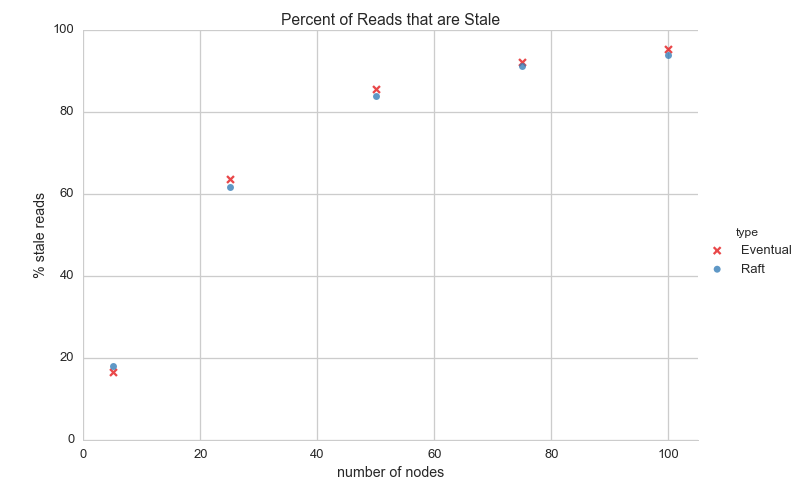
\includegraphics[width=\textwidth]{hcfigures/stale_reads.png}
        \caption{\textsf{Eventual has marginally more stale reads than Raft at higher nodes, but the majority of reads in both systems are stale at even moderate system sizes. Instead of looking at the full visibility latency to suggest how long objects will be stale, I propose we instead look at the maximally replicated latency as shown in Figure \ref{fig:partial_visibility_latency}.}}
        \label{fig:stale_reads}
\end{figure}

\begin{figure}[!h]
    \centering
        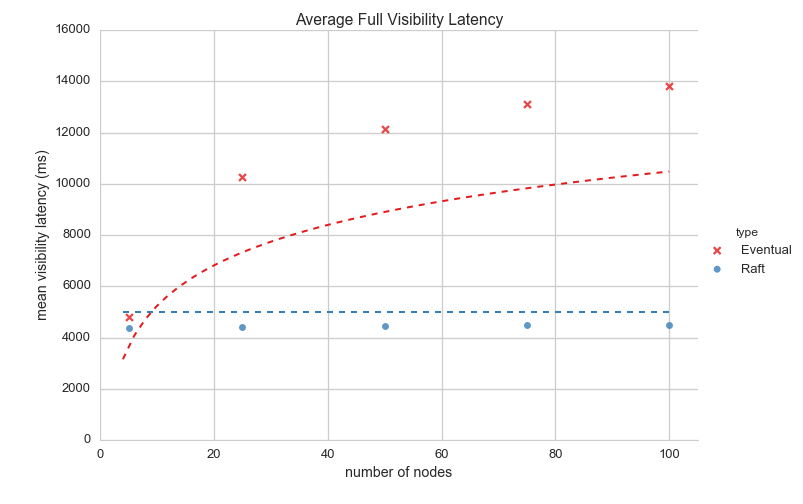
\includegraphics[width=\textwidth]{hcfigures/visibility_latency.png}
        \caption{\textsf{This graph measures the latency for a write to become fully visible (therefore excluding partially replicated writes). The lines given are the estimates for convergence given the number of nodes and the timing parameter. The blue line for Raft represents the heartbeat interval, real times are slightly lower due to writes that arrive at the leader right before an \texttt{AppendEntries}. The red line for eventual is an underestimate since it assumes optimal neighbor selection (every node always selects a neighbor that doesn't have the write being propagated).}}
        \label{fig:visibility_latency}
\end{figure}

\begin{figure}[!h]
    \centering
        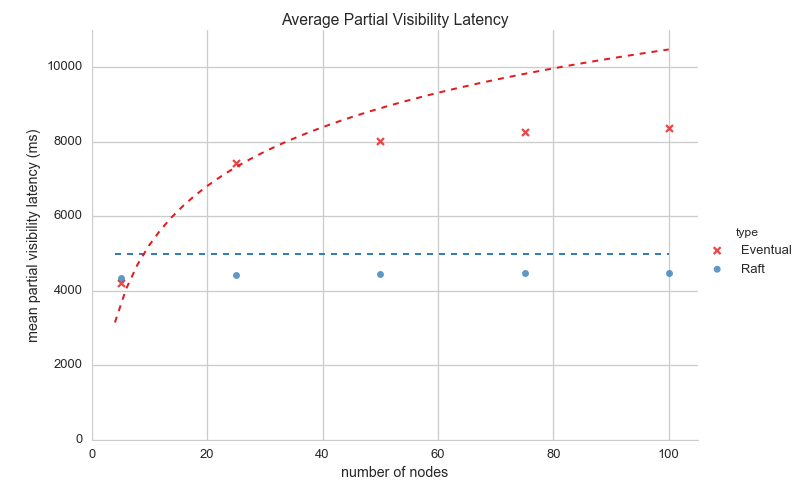
\includegraphics[width=\textwidth]{hcfigures/partial_visibility_latency.png}
        \caption{\textsf{This graph shows the average latency for a write to become maximally visible (e.g. the mean amount of time it took for a write to be replicated, even partially). The lines are the same convergence estimates as shown in Figure \ref{fig:visibility_latency}. Raft has no partial visibility, a write is either fully replicated or dropped, therefore it's latency is the same. Eventual however does allow partial visibility; the more nodes in the system, the lower the replication percent, and therefore the lower the convergence time.}}
        \label{fig:partial_visibility_latency}
\end{figure}

\begin{figure}[!h]
    \centering
        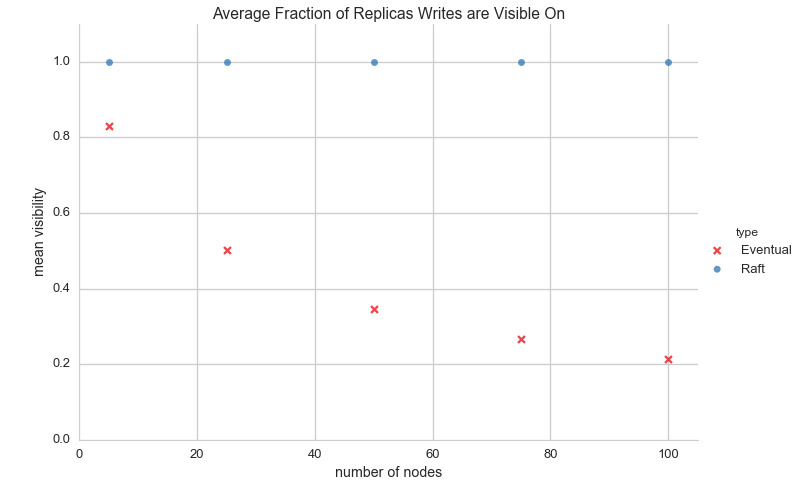
\includegraphics[width=\textwidth]{hcfigures/mean_visibility.png}
        \caption{\textsf{This metric shows the average replication for writes, where replication is defined as the ratio between the number of replicas the write is visible on to the total number of replicas. A write won't become fully replicated in Eventual if it is stomped on by a later write and not propagated. The more nodes in the system, the greater the likelihood of stomping because full replication will take longer.}}
        \label{fig:mean_visibility}
\end{figure}


\begin{figure}[!h]
    \centering
        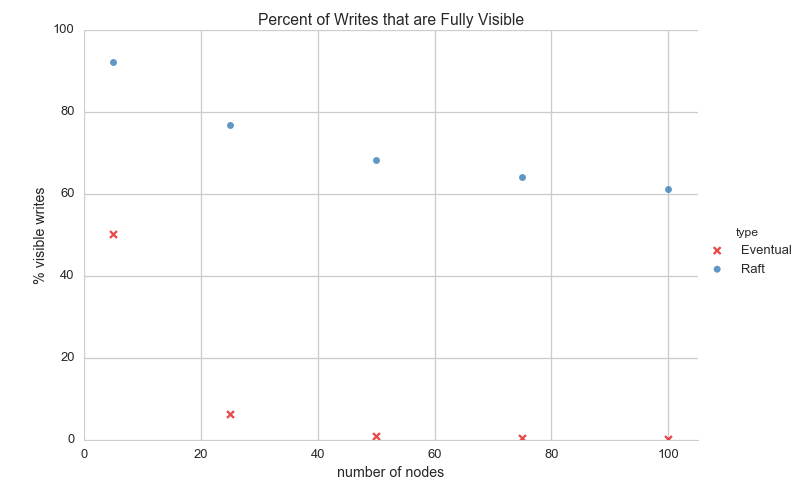
\includegraphics[width=\textwidth]{hcfigures/visible_writes.png}
        \caption{\textsf{This metric shows the percent of writes that become fully visible in the system. Because the full visibility decreases exponentially with more nodes, I propose that we cannot use the full visibility latency metric to understand how stale reads and forks happen in the system, but must instead use the mean maximal visibility latency metric which shows that Raft and Eventual are much closer.}}
        \label{fig:visible_writes}
\end{figure}

% \begin{figure}[!h]
%     \centering
%         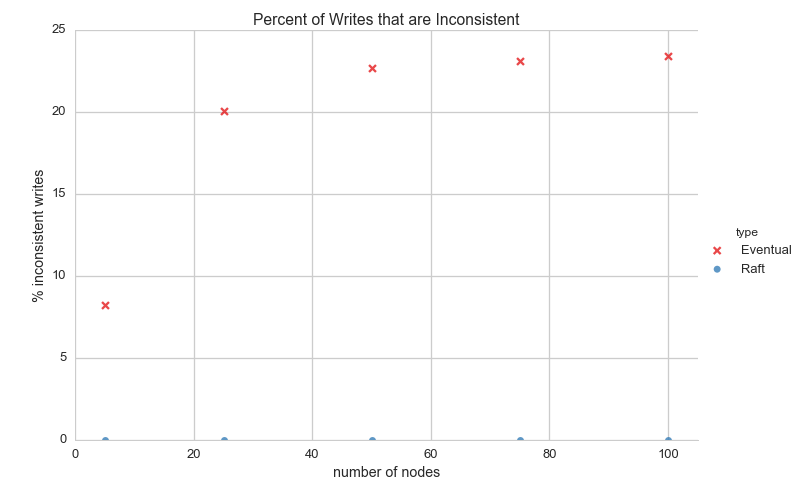
\includegraphics[width=\textwidth]{hcfigures/inconsistent_writes.png}
%         \caption{\textsf{Raft will not allow an inconsistent write by dropping it, however every Eventual fork is an inconsistent write.}}
%         \label{fig:inconsistent_writes}
% \end{figure}
%
% \begin{figure}[!h]
%     \centering
%         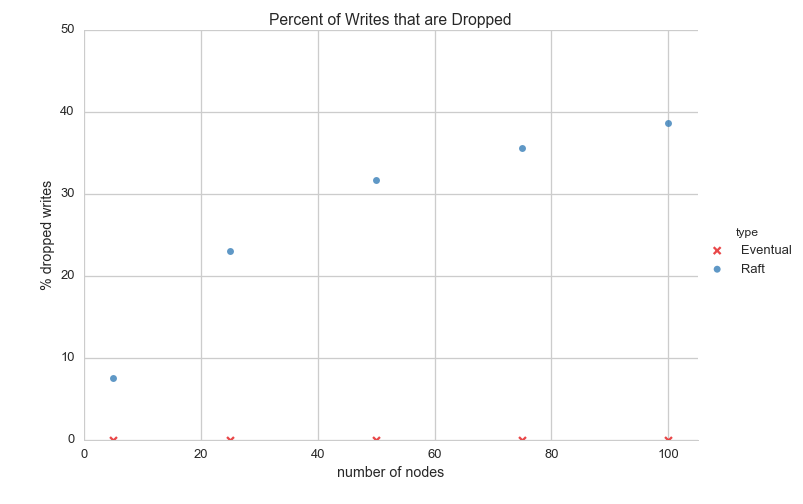
\includegraphics[width=\textwidth]{hcfigures/dropped_writes.png}
%         \caption{\textsf{Raft should drop 100\% of its forks, Eventual drops none.}}
%         \label{fig:dropped_writes}
% \end{figure}

\begin{figure}[!h]
    \centering
        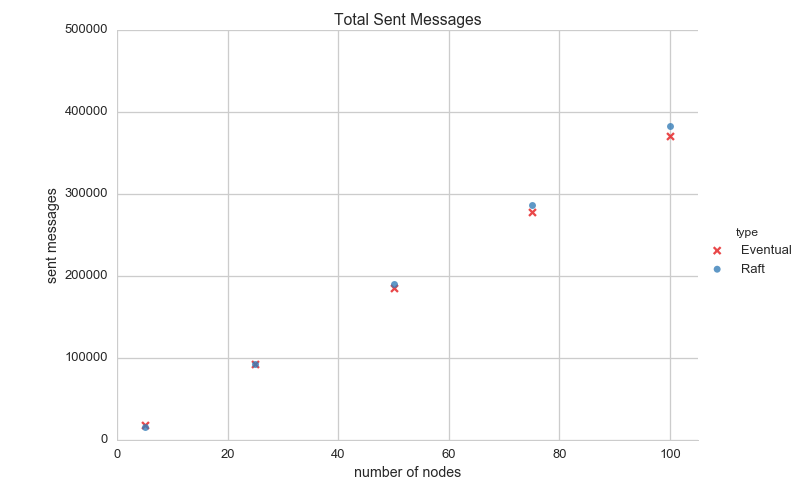
\includegraphics[width=\textwidth]{hcfigures/messages_sent.png}
        \caption{\textsf{In these simulations both Raft and Eventual have a fixed communication budget that is defined by the relationship of their timing parameters (anti-entropy delay and heartbeat interval).\\
\\
\\}}
        \label{fig:messages_sent}
\end{figure}

\begin{figure}[!h]
    \centering
        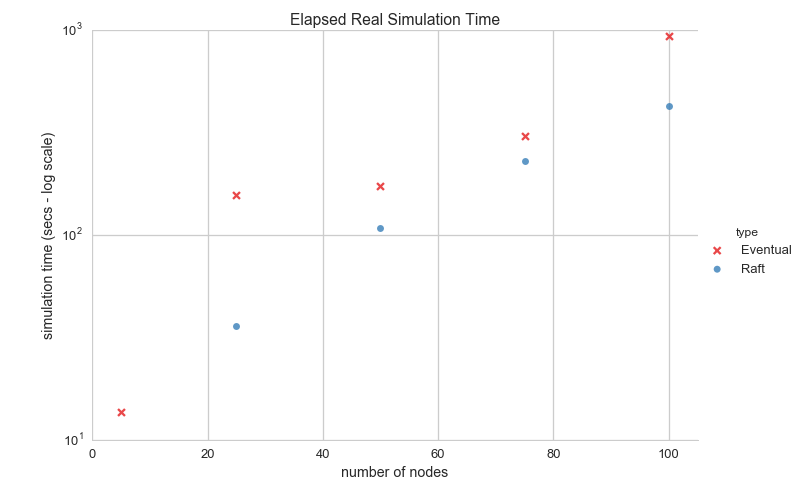
\includegraphics[width=\textwidth]{hcfigures/simulation_time.png}
        \caption{\textsf{Reducing the number of objects in the simulation greatly improved the performance!}}
        \label{fig:simulation_time}
\end{figure}

% \begin{figure}[!h]
%     \centering
%         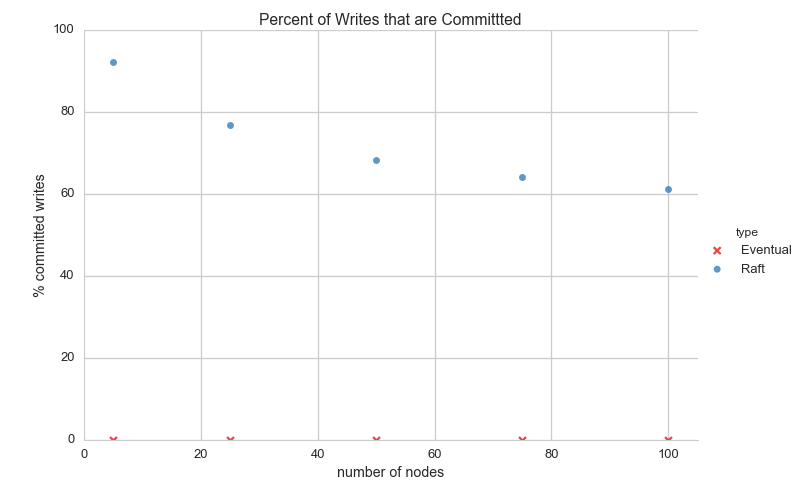
\includegraphics[width=\textwidth]{hcfigures/committed_writes.png}
%         \caption{\textsf{Raft commits nearly all writes (except those that it drops). Eventual commits none.}}
%         \label{fig:committed_writes}
% \end{figure}
%
% \begin{figure}[!h]
%     \centering
%         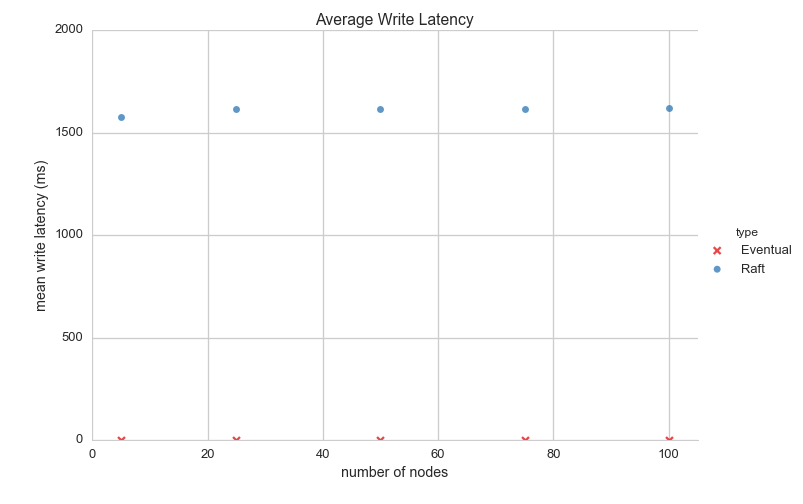
\includegraphics[width=\textwidth]{hcfigures/write_latency.png}
%         \caption{\textsf{The write latency embeds the amount of time for a \texttt{RemoteWrite} to the leader and the response. Eventual writes locally, immediately therefore there is no write latency.}}
%         \label{fig:write_latency}
% \end{figure}
%
% \begin{figure}[!h]
%     \centering
%         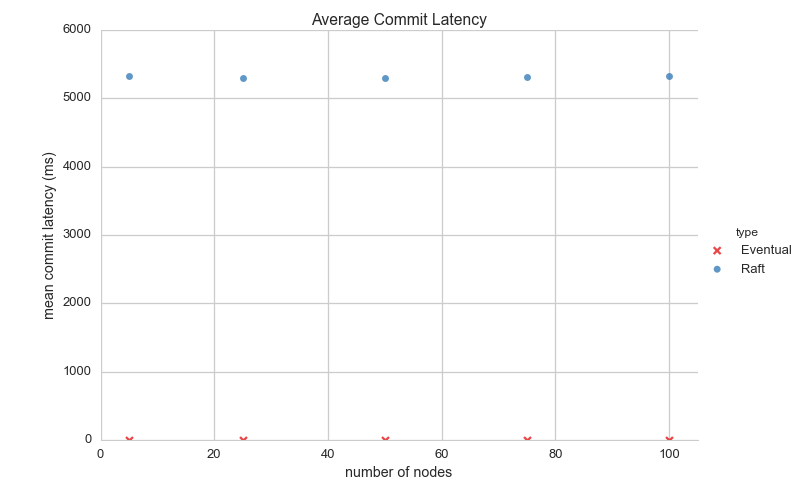
\includegraphics[width=\textwidth]{hcfigures/commit_latency.png}
%         \caption{\textsf{The commit latency is approximately the remote write latency plus a heartbeat interval, given no outages.}}
%         \label{fig:commit_latency}
% \end{figure}
%
% \begin{figure}[!h]
%     \centering
%         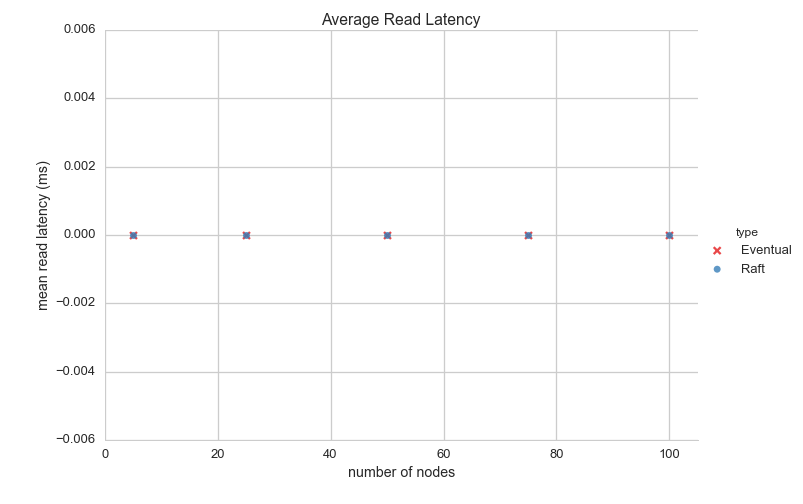
\includegraphics[width=\textwidth]{hcfigures/read_latency.png}
%         \caption{\textsf{Every node implements read local cache, therefore every node has zero read latency.}}
%         \label{fig:read_latency}
% \end{figure}
%
% \begin{figure}[!h]
%     \centering
%         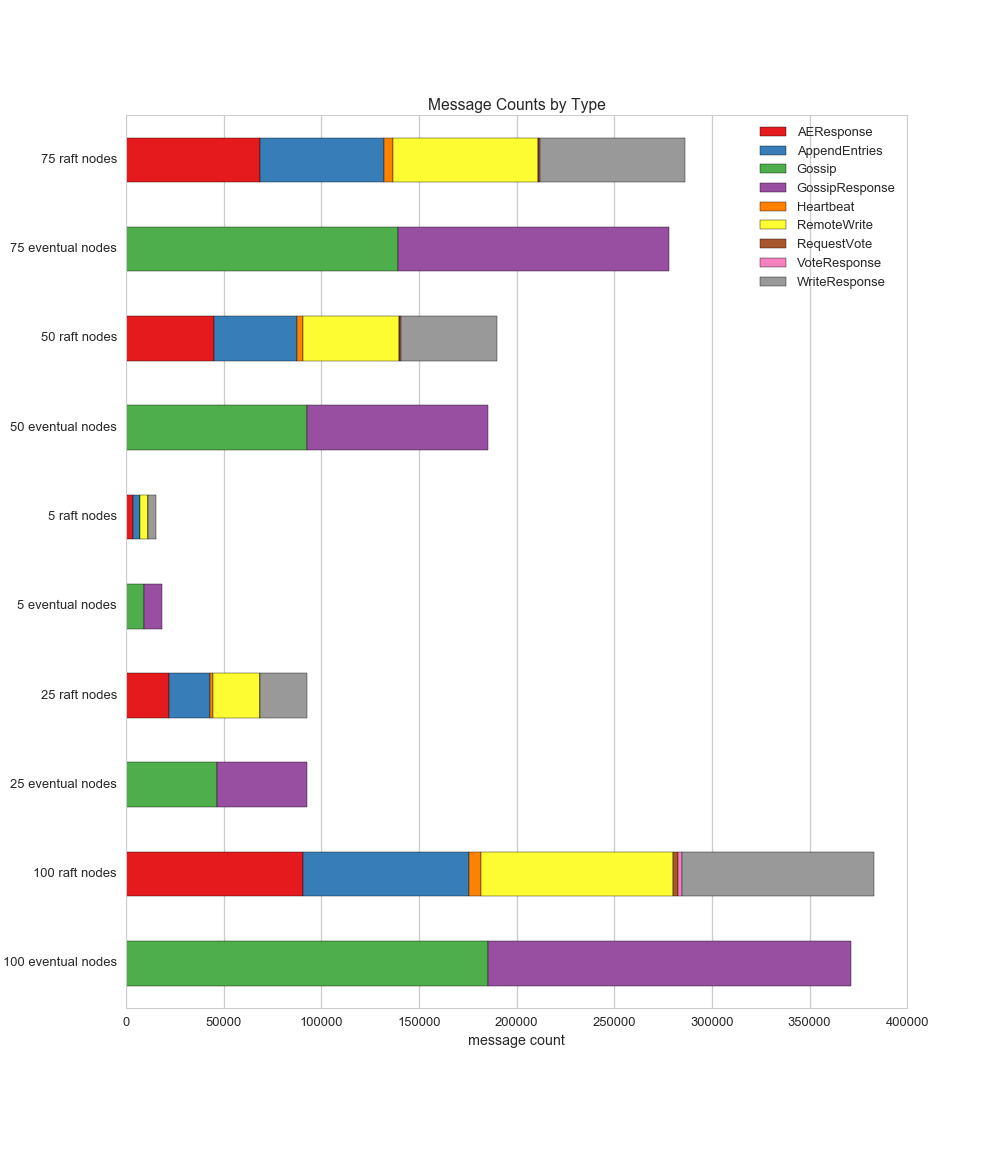
\includegraphics[height=.9\textheight]{hcfigures/message_counts.png}
%         \caption{\textsf{See \ref{fig:messages_sent} for more details.}}
%         \label{fig:message_counts}
% \end{figure}

\begin{table}[!h]
\makebox[\textwidth][c]{
\centering
\begin{tabular}{|r|ll|}
\hline
setting              & raft                      & eventual                  \\
\hline
Nodes                & 5, 25, 50, 75, 100        & 5, 25, 50, 75, 100        \\
Links                & 20, 600, 2450, 9900, 5550 & 20, 600, 2450, 9900, 5550 \\
Local Latency ($\mu$, $\sigma$) & (100, 5)       & (100, 5)                  \\
Wide Latency ($\mu$, $\sigma$) & (1000, 56)      & (1000, 56)                \\
Latency Range        & 888-1112ms                & 888-1112ms                \\
Tick Metric $T$      & 10000                     & 10000                     \\
Tick Model           & bailis                    & bailis                    \\
Election Timeout     & U(10000, 20000)           & N/A                       \\
Heartbeat Interval   & 5000ms                    & N/A                       \\
Anti-Entropy Delay   & N/A                       & 2500ms                    \\
AE Neighbors ($n$)   & N/A                       & 1                         \\
$P_{sync}$           & N/A                       & N/A                       \\
$P_{local}$          & N/A                       & 0.6                       \\
$P_{conflict}$       & 0.8                       & 0.8                       \\
$P_{read}$           & 0.5                       & 0.5                       \\
Access Interval ($\mu$, $\sigma$) & (1800, 240)  & (1800, 240)               \\
Objects              & 17                        & 17                        \\
Access per Object    & 240                       & 240                       \\
Writes               & 12,015 - 240,045          & 12,015 - 240,045          \\
\hline
\end{tabular}}
\caption{\textsf{Static settings aggregated by Replica/Experiment type.}}
\label{table:settings}
\end{table}

\end{document}
